\documentclass[a4paper,11pt]{article}

% ----------------- Encoding & language -----------------
\usepackage[utf8]{inputenc}
\usepackage[T1]{fontenc}
\usepackage[english]{babel}

% ----------------- Geometry & layout -----------------
\usepackage[a4paper,margin=1.8cm]{geometry} % narrow margins

\usepackage{setspace}
\onehalfspacing
\usepackage{microtype}
\usepackage{parskip} % no paragraph indents

% ----------------- Fonts (modern, clean) -----------------
\usepackage{lmodern}
\renewcommand{\familydefault}{\sfdefault} % sans-serif default

% ----------------- Colors & links -----------------
\usepackage{xcolor}
\definecolor{accent}{HTML}{0077B6}      % main accent (blue)
\definecolor{accentlight}{HTML}{E0F4FF} % light accent background
\definecolor{textgray}{gray}{0.25}

\usepackage{tikz}
\usetikzlibrary{positioning,shadows.blur}
\usepackage{float}


\usepackage{array}
\usepackage{booktabs}

\definecolor{tblhead}{gray}{0.9} % header background color

% left-aligned paragraph column
\newcolumntype{L}[1]{>{\raggedright\arraybackslash}p{#1}}

% For code listings
\usepackage{minted}   % remember: compile with -shell-escape




\usepackage{hyperref}
\hypersetup{
	colorlinks=true,
	linkcolor=accent,
	urlcolor=accent,
	citecolor=accent
}

% ----------------- Section styling -----------------
\usepackage{titlesec}


% section numbers up to subsubsection
\setcounter{secnumdepth}{3}
\setcounter{tocdepth}{3}

\titleformat{\section}
{\large\bfseries\color{textgray}}
{\thesection}
{0.7em}
{}
[\color{accent}\titlerule] % colored rule under section title

\titleformat{\subsection}
{\normalsize\bfseries\color{accent}}
{\thesubsection}
{0.7em}
{}

\titleformat{\subsubsection}
{\normalsize\itshape\color{textgray}}
{\thesubsubsection}
{0.7em}
{}

% ----------------- Header / footer -----------------
\usepackage{fancyhdr}
\pagestyle{fancy}
\fancyhf{}
\lhead{\small Challenger RP2040 UWB Progress}
\rhead{\small Siddharth Patel}
\cfoot{\thepage}
\renewcommand{\headrulewidth}{0.3pt}
\renewcommand{\footrulewidth}{0pt}

% ----------------- Boxes & misc -----------------
\usepackage[skins]{tcolorbox}
\tcbuselibrary{breakable}

\tcbset{
	sharp corners,
	boxrule=0pt,
	colback=white,
}

% Optional: code listings later
% \usepackage{minted}

% ----------------- Title data -----------------
\title{\vspace{-1.5cm}\bfseries\Huge Challenger RP2040 UWB (DWM3000)\\[0.4em]
	\Large Progress Documentation}
\author{\large Siddharth Patel}
\date{\today}

\begin{document}
	
	% ----------------- Custom first page -----------------
	\begin{titlepage}
		\color{textgray}
		\vspace*{1cm}
		
		% Top colored bar
		\begin{tcolorbox}[colback=accent, height=0.4cm, boxrule=0pt, enlarge left by=-1.8cm, enlarge right by=-1.8cm]
		\end{tcolorbox}
		
		\vspace{1.5cm}
		
		{\Huge\bfseries Challenger RP2040 UWB (DWM3000)\\[0.5em]
			\LARGE Progress Documentation}
		
		\vspace{1.2cm}
		
		{\Large Siddharth Patel}\\[0.4cm]
		{\large HTW Berlin}
		
		\vspace{1.8cm}
		
		\begin{tcolorbox}[
			colback=accentlight,
			boxrule=0pt,
			enlarge left by=0cm,
			enlarge right by=0cm,
			left=8pt, right=8pt, top=8pt, bottom=8pt
			]
			\textbf{Document Summary}\\[0.4em]
			This document tracks the steps taken to bring up the iLabs Challenger RP2040 UWB board,
			program it using the Arduino toolchain, run initial UWB examples, and explore how distance
			data can be integrated into a larger robotics system (e.g.\ Raspberry Pi 5).
		\end{tcolorbox}
		
		\vfill
		
		\begin{tabular}{ll}
			\textbf{Board} & iLabs Challenger RP2040 UWB (DWM3000) \\
			\textbf{UWB Chip} & Qorvo DW3000 (DWM3000 module) \\
			\textbf{Main MCU} & Raspberry Pi RP2040 \\
			\textbf{Toolchain} & Arduino IDE (RP2040 core) \\
			\textbf{Date} & \today \\
		\end{tabular}
		
		\vspace{1cm}
		
		% Bottom colored bar
		\begin{tcolorbox}[colback=accent, height=0.25cm, boxrule=0pt, enlarge left by=-1.8cm, enlarge right by=-1.8cm]
		\end{tcolorbox}
	\end{titlepage}
	
	% ----------------- TOC -----------------
	\tableofcontents
	\listoffigures
	\listoftables
	\clearpage
	
%	% ====================================================
%	\section{Introduction}
%	% Short context + goal of this document.
	
% ================================
\section{Programming Options for the Challenger RP2040 UWB}
\label{sec:programming-options}
% ================================

\subsection{RP2040 + DWM3000: Board Overview}

The \emph{Challenger RP2040 UWB} from iLabs combines
\[
{Challenger RP2040 UWB} \;=\; {RP2040 (MCU)} \;+\; {DWM3000 (UWB)}.
\]

The RP2040 defines how we can program the board, while the DWM3000 defines which UWB libraries we can actually use.

\begin{figure}[H]
	\centering
	% include the standalone illustration PDF
	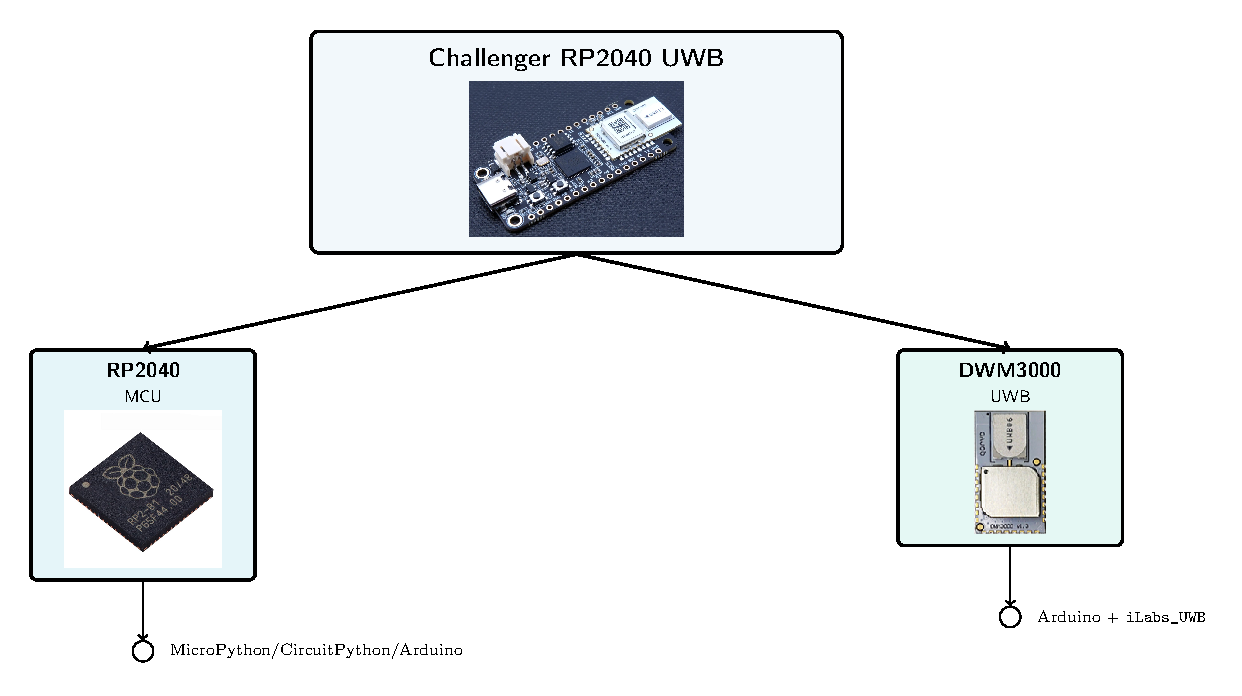
\includegraphics[width=0.9\linewidth]{rp2040_dwm3000_illustration/rp2040_dwm3000_illustration}% 
	% or: {figures/rp2040_dwm3000_illustration}
	\caption{Conceptual view of the Challenger RP2040 UWB: RP2040 MCU, DWM3000 UWB module and their firmware options.}
	\label{fig:rp2040-dwm3000-options}
\end{figure}


\subsection{Firmware Options on the RP2040}

Because the RP2040 is the same MCU used on the Raspberry Pi Pico, it can in principle be programmed with:\vspace{-0.25em}
\begin{itemize}
	\item \textbf{MicroPython}\footnote{\url{https://micropython.org/download/?mcu=rp2040}}
	\item \textbf{CircuitPython}\footnote{\url{https://circuitpython.org/board/raspberry_pi_pico/}}
	\item \textbf{Arduino (C++ with Arduino IDE)}\footnote{\url{https://ilabs.se/getting-your-challenger-rp2040-board-up-and-running-with-the-arduino-ide/}}
\end{itemize}

\subsection{Library Support for the DWM3000}

For the UWB part, the situation is much more restricted:

\begin{itemize}
	\item The iLabs product page notes that, although the board is compatible with CircuitPython, \emph{“to date there does not exist a support library in Python for the DWM3000 module.”}\footnote{\url{https://ilabs.se/product/challenger-rp2040-uwb/}}
	\item iLabs provides an official \textbf{Arduino library} and examples for the DWM3000 via the \texttt{iLabs\_UWB} repository.\footnote{\url{https://github.com/PontusO/iLabs_UWB}}
\end{itemize}

\subsection{Conclusion for This Project}

Because only the Arduino ecosystem currently offers a maintained UWB library for the DWM3000, all experiments in this document are based on:
\[
{RP2040 firmware} \;=\; \textbf{Arduino language + Arduino IDE + \texttt{iLabs\_UWB} library}.
\]

MicroPython and CircuitPython remain theoretical options for the RP2040 itself, but are not used here due to the missing DWM3000 support.

	
	
	
	
\newpage
	
% ====================================================
\section{Arduino-Based Workflow for the Challenger RP2040 UWB}
\label{sec:arduino-workflow}
% ====================================================

\subsection{Following the iLabs Getting-Started Guide}
\label{subsec:ilabs-guide}

The official starting point for programming the Challenger RP2040 UWB is the iLabs
Arduino guide.\footnote{\url{https://ilabs.se/getting-your-challenger-rp2040-board-up-and-running-with-the-arduino-ide/}}
It explains how to install the iLabs board package and select the correct board in the Arduino IDE.

\begin{tcolorbox}[title=Basic setup (summary),colback=accentlight!60!white]
	\begin{enumerate}
		\item Install the iLabs RP2040 board package in the Arduino IDE as described in the guide.
		\item In \texttt{Tools} $\rightarrow$ \texttt{Board}, select \texttt{iLabs Challenger 2040 UWB}.
		\item Verify that a serial port for the board (e.g.\ \texttt{/dev/cu.usbmodemXXXX}) is visible.
	\end{enumerate}
\end{tcolorbox}

\begin{figure}[H]
	\centering
	\includegraphics[width=0.75\linewidth]{figures/board_port_selection}%
	\caption{Selecting the \texttt{iLabs Challenger 2040 UWB} board and USB serial port in the Arduino IDE.}
	\label{fig:board-port-selection}
\end{figure}

% ----------------------------------------------------
\subsection{Bootloader Issue: ``No Drive Detected''}
\label{subsec:no-drive}

When uploading directly from the Arduino IDE, the RP2040 bootloader is supposed to
mount as a USB drive. On macOS this sometimes fails and the IDE reports:

\begin{figure}[H]
	\centering
	\includegraphics[width=0.7\linewidth]{figures/no_drive_error}%
	\caption{Typical Arduino upload error when the RP2040 UF2 drive is not detected.}
	\label{fig:no-drive-error}
\end{figure}

To work around this, sketches are uploaded via a \texttt{.uf2} file and manual drag\&drop.

% ----------------------------------------------------
\subsection{Programming via UF2 Files}
\label{subsec:uf2-programming}

The UF2 method separates two things:
\begin{enumerate}
	\item the Arduino IDE \emph{compiles} a \texttt{.uf2} file, and
	\item the Mac \emph{copies} that file to the RP2040 boot drive.
\end{enumerate}

\subsubsection{One-time setup in the Arduino IDE}

\begin{tcolorbox}[title=Step 1: IDE configuration,colback=accentlight!60!white]
	\begin{enumerate}
		\item Open your sketch in the Arduino IDE.
		\item In \texttt{Tools} set:
		\begin{itemize}
			\item \texttt{Board} $\rightarrow$ \texttt{iLabs Challenger 2040 UWB},
			\item \texttt{Upload Method} $\rightarrow$ \texttt{Default (UF2)},
			\item \texttt{USB Stack} $\rightarrow$ \texttt{Pico SDK}.
		\end{itemize}
		\item Choose \texttt{Sketch} $\rightarrow$ \texttt{Export compiled Binary}.
		\item Open \texttt{Sketch} $\rightarrow$ \texttt{Show Sketch Folder} and locate the
		generated \texttt{.uf2} file (e.g.\ \texttt{my\_sketch.ino.uf2}).
	\end{enumerate}
\end{tcolorbox}

\subsubsection{Put the board into BOOTSEL mode}

\begin{tcolorbox}[title=Step 2: Enter BOOTSEL mode,colback=accentlight!60!white]
	\begin{enumerate}
		\item Unplug the USB cable from the Challenger RP2040 UWB.
		\item Hold the \textbf{BOOT} button and plug the USB cable back in.
		\item Release \textbf{BOOT} when a new USB drive named \texttt{RPI-RP2} appears on the Mac.
	\end{enumerate}
\end{tcolorbox}

\subsubsection{Upload the program via UF2}

\begin{tcolorbox}[title=Step 3: Copy UF2 file,colback=accentlight!60!white]
	\begin{enumerate}
		\item Drag the \texttt{.uf2} file from the sketch folder onto the \texttt{RPI-RP2} drive in Finder.
		\item Wait until \texttt{RPI-RP2} automatically ejects.
		\item Unplug and reconnect the board in normal mode. The new sketch is now running.
	\end{enumerate}
\end{tcolorbox}

% ----------------------------------------------------
\subsection{FreeRTOS Configuration Error}
\label{subsec:freertos-error}

Some UWB example sketches use FreeRTOS on the RP2040. If FreeRTOS is not enabled,
compilation fails with an error similar to:

\begin{figure}[H]
	\centering
	\includegraphics[width=0.7\linewidth]{figures/freertos_error}%
	\caption{Compilation error when FreeRTOS is not enabled for the Challenger RP2040 UWB.}
	\label{fig:freertos-error}
\end{figure}

\subsubsection{Enable FreeRTOS for the Challenger RP2040 UWB}

\begin{tcolorbox}[title=Fix: enable FreeRTOS,colback=accentlight!60!white]
	\begin{enumerate}
		\item Open the example sketch (e.g.\ \texttt{ex\_01a\_simple\_tx.ino}) in the Arduino IDE.
		\item In \texttt{Tools} set:
		\begin{itemize}
			\item \texttt{Board} $\rightarrow$ \texttt{iLabs Challenger 2040 UWB},
			\item \texttt{Upload Method} $\rightarrow$ \texttt{Default (UF2)},
			\item \texttt{USB Stack} $\rightarrow$ \texttt{Pico SDK},
			\item \texttt{Operating System} $\rightarrow$ \textbf{FreeRTOS SMP}.
		\end{itemize}
		\item Compile again with \texttt{Sketch} $\rightarrow$ \texttt{Verify/Compile}.
		\item If compilation succeeds, upload the sketch via the UF2 workflow described above.
	\end{enumerate}
\end{tcolorbox}

\newpage

	% ====================================================
% ====================================================
\section{Which Data Can We Get from the DWM3000?}
\label{sec:uwb-data}
% ====================================================

\subsection{Raw data directly from the DWM3000}

When the RP2040 talks to the DWM3000 over SPI, it can read several types of
\emph{raw} information from the chip registers.\footnote{Full details are in the
	DWM3000 datasheet: \url{https://www.qorvo.com/products/p/DWM3000\#documents}}

\begin{table}[h]
	\centering
	\caption{Typical raw data available from the DWM3000}
	\label{tab:uwb-raw-data-simple}
	\begin{tabular}{p{0.9\linewidth}}
		\toprule
		\textbf{Raw data type (examples)} \\
		\midrule
		RX and TX timestamps in the internal UWB clock \\
		Received UWB frame bytes (header fields and payload) \\
		Channel impulse response (CIR) samples \\
		RX quality and diagnostic values (power, noise, CRC status, \dots) \\
		Status and interrupt flags (RXOK, timeout, errors, \dots) \\
		\bottomrule
	\end{tabular}
\end{table}

These low-level values are the building blocks. From them we can compute things
like time-of-flight, distance or more advanced metrics.

% ----------------------------------------------------
\subsection{Derived data on RP2040 using the UWB library}
\label{subsec:uwb-derived-data}

With the iLabs UWB library running on the RP2040, these raw values are turned
into more convenient, \emph{processed} data structures:

\begin{table}[h]
	\centering
	\caption{Examples of derived data on the RP2040}
	\label{tab:uwb-rp2040-data-simple}
	\begin{tabular}{p{0.9\linewidth}}
		\toprule
		\textbf{Processed data (examples)} \\
		\midrule
		Distance between two nodes (single range result in m or mm) \\
		Simple range quality or “RSSI” value per distance measurement \\
		Logged packets that combine payload, timestamps and diagnostics \\
		2D or 3D position estimates of a tag based on multiple ranges \\
		Debug recordings of CIR, timestamps and error counters \\
		\bottomrule
	\end{tabular}
\end{table}

	
	\newpage
	
	% ====================================================
	% ====================================================
	\section{Retrieving Raw UWB Data on the RP2040}
	\label{sec:raw-data-demo}
	% ====================================================
	
	
	\subsection{How to run the raw-data demo}
	
	\begin{tcolorbox}[title=Step-by-step setup,colback=accentlight!60!white,sharp corners]
		\begin{enumerate}
			\item \textbf{Board A (RX)}:  
			Flash \texttt{rx\_raw\_data\_demo.ino} to the first Challenger RP2040 UWB  
			(using the Arduino + UF2 workflow from Section~\ref{sec:arduino-workflow}).
			\item Open the Arduino \textbf{Serial Monitor} for Board A with the baudrate
			used in the sketch (e.g.\ 115200~Bd).
			\item \textbf{Board B (TX)}:  
			Flash a TX example sketch, e.g.\ \texttt{ex\_01a\_simple\_tx.ino} from the
			iLabs examples.\footnote{\url{https://github.com/PontusO/iLabs_UWB/blob/main/examples/ex_01a_simple_tx/ex_01a_simple_tx.ino}}
			\item Power both boards.  
			Board B periodically sends UWB frames; Board A prints one raw dump for
			every received frame.
		\end{enumerate}
	\end{tcolorbox}
	
	\subsection{Example serial output}
	
	The TX board simply reports that frames are being sent, while the RX board prints
	a full raw dump for each frame (status, frame bytes, RX timestamp, CIR, power
	values, \dots).
	
	\begin{figure}[H]
		\centering
		\begin{minipage}[t]{0.25\linewidth}
			\centering
			\includegraphics[width=\linewidth]{figures/tx_frames_sent}% <- your TX screenshot
			\caption*{TX board: simple ``TX Frame Sent'' log from \texttt{ex\_01a\_simple\_tx.ino}.}
		\end{minipage}\hspace{2.5cm}
		\begin{minipage}[t]{0.45\linewidth}
			\centering
			\includegraphics[width=\linewidth]{figures/rx_raw_dump}% <- your RX screenshot
			\caption*{RX board: raw frame dump from \texttt{rx\_raw\_data\_demo.ino} (timestamps, CIR, diagnostics).}
		\end{minipage}
		\caption{Serial output of the TX example (left) and the raw-data receiver demo (right).}
		\label{fig:raw-data-demo-output}
	\end{figure}
	
	
	\newpage
	
		\subsection{Sketch: \texttt{rx\_raw\_data\_demo.ino}}
	
	The sketch \texttt{rx\_raw\_data\_demo.ino} configures the Challenger RP2040 UWB
	as a receiver and prints the raw information from every incoming UWB frame
	(timestamps, frame bytes, CIR, diagnostics, \dots) to the serial console.
	
	\begin{tcolorbox}[colback=black!2,
		boxrule=0.3pt,
		sharp corners,
		breakable,
		left=6pt,right=6pt,top=6pt,bottom=6pt]
		\inputminted[
		fontsize=\small,
		breaklines,
		linenos
		]{c++}{rx_raw_data_demo/rx_raw_data_demo.ino}
	\end{tcolorbox}
	
	\newpage
	
	% ====================================================
	\section{Example: Distance Measurement Between Two Nodes}
	\label{sec:distance-measurement}
	% ====================================================
	
	For a first end–to–end distance test we used the single–sided two–way ranging
	(SS~TWR) examples from the iLabs UWB library:
	
	\begin{itemize}
		\item \textbf{Node A (initiator)}: \texttt{ex\_06a\_ss\_twr\_initiator.ino}\footnote{\url{https://github.com/PontusO/iLabs_UWB/blob/main/examples/ex_06a_ss_twr_initiator/ex_06a_ss_twr_initiator.ino}}
		\item \textbf{Node B (responder)}: \texttt{ex\_06b\_ss\_twr\_responder.ino}\footnote{\url{https://github.com/PontusO/iLabs_UWB/blob/main/examples/ex_06b_ss_twr_responder/ex_06b_ss_twr_responder.ino}}
	\end{itemize}
	
	The responder replies to each poll frame, and the initiator computes the
	time-of-flight and prints the resulting distance in meters on the serial
	console (Figure~\ref{fig:ss-twr-distance}).
	
	\begin{figure}[h]
		\centering
		\includegraphics[width=0.7\linewidth]{figures/ss_twr_distance_output}% <- replace with your screenshot filename
		\caption{Serial output of \texttt{ex\_06a\_ss\_twr\_initiator.ino} showing repeated distance estimates between the two nodes.}
		\label{fig:ss-twr-distance}
	\end{figure}
	
	\newpage
%	% ====================================================
%	\section{Conclusion and Outlook}
%	\label{sec:conclusion}
%	% ====================================================
%	
%	Table~\ref{tab:conclusion-summary} summarizes the progress made so far with the
%	Challenger RP2040 UWB board.
%	
%	\begin{table}[H]
%		\centering
%		\caption{Summary of steps completed in this work}
%		\label{tab:conclusion-summary}
%		\begin{tabular}{p{4cm} p{9cm}}
%			\toprule
%			\textbf{Step} & \textbf{What was achieved} \\
%			\midrule
%			Hardware + firmware choice
%			& Identified the Challenger RP2040 UWB as \textbf{RP2040 + DWM3000} and selected the \textbf{Arduino + iLabs\_UWB} toolchain as the only practical option with a maintained DWM3000 library. \\[0.3em]
%			
%			Arduino workflow
%			& Set up a reliable upload workflow using \textbf{UF2 binaries}, documented the ``No drive to deploy'' issue, BOOTSEL mode, and the required \textbf{FreeRTOS SMP} setting. \\[0.3em]
%			
%			Raw data access
%			& Implemented and ran \texttt{rx\_raw\_data\_demo.ino} to print \textbf{raw UWB data} (frame bytes, timestamps, CIR, diagnostics) from the DWM3000 on the serial console. \\[0.3em]
%			
%			Data types
%			& Distinguished between \textbf{raw chip data} (directly from DWM3000 registers) and \textbf{derived data} on the RP2040 (distance, quality metrics, logs, localisation state). \\[0.3em]
%			
%			Distance demo
%			& Used the \texttt{ex\_06a\_ss\_twr\_initiator} and \texttt{ex\_06b\_ss\_twr\_responder} examples to obtain \textbf{live distance measurements} between two nodes and verify end-to-end ranging. \\
%			\bottomrule
%		\end{tabular}
%	\end{table}
%	
%	Future work can build on this foundation: forwarding distances to a Raspberry~Pi,
%	testing multi-anchor setups, and experimenting with full 2D/3D localisation.
	
	
	
	
%	\section{Example: Distance Measurement Between Two Nodes}
%	\label{sec:distance-measurement}
%	
%	\subsection{Ranging Mode (e.g.\ Single-Sided Two-Way Ranging)}
%	\label{subsec:ranging-mode}
%	% Concept of SS-TWR, initiator, responder.
%	
%	\subsection{Distance Retrieval Example Sketch}
%	\label{subsec:distance-sketch}
%	% Where distance is calculated and printed in the example code.
%	
%	\subsection{Observed Output and Behaviour}
%	\label{subsec:distance-output}
%	% Serial logs, LED behaviour, stability of readings.
%	
%	% ====================================================
%	\section{Potential Data Flows and System-Level Use Cases}
%	\label{sec:potential-data}
%	
%	\subsection{Forwarding UWB Data to a Host Processor}
%	\label{subsec:data-forwarding}
%	% UART, USB-Serial, I2C to Raspberry Pi 5, etc.
%	
%	\subsection{Anchor and Tag System Design}
%	\label{subsec:anchor-tag}
%	% Static anchors, mobile tag, multilateration ideas.
%	
%	\subsection{Towards 3D Position and Orientation}
%	\label{subsec:3d-pos-ori}
%	% Combine UWB with IMU, depth camera, etc.
%	
%	% ====================================================
%	\section{Next Steps}
%	\label{sec:next-steps}
%	
%	\subsection{Firmware Refinements}
%	% Cleaner abstraction, parameterization, error handling.
%	
%	\subsection{Integration with Robot / SolarSwarm Platform}
%	% High-level architecture of how UWB module fits into system.
%	
%	\subsection{Planned Experiments}
%	% Multi-anchor tests, moving robot, logging, performance metrics.
%	
	% ====================================================
%	\section*{References}
%	\addcontentsline{toc}{section}{References}
	
%	% You can later replace this with a BibTeX file if you want.
%	\begin{thebibliography}{9}
%		
%		\bibitem{qorvo_dw3000_um}
%		Qorvo,
%		\emph{DW3000 User Manual}, 2021.
%		
%		\bibitem{qorvo_dw1000_um}
%		Qorvo,
%		\emph{DW1000 User Manual}, 2017.
%		
%		\bibitem{ilabs_uwb_repo}
%		P.~Olsson,
%		\emph{iLabs\_UWB: A support library for the Challenger RP2040 UWB boards},
%		GitHub repository, 2025.
%		
%		\bibitem{challenger_rp2040_product}
%		iLabs,
%		\emph{Challenger RP2040 UWB (DWM3000) product page},
%		online resource.
%		
%		\bibitem{ilabs_getting_started}
%		iLabs,
%		\emph{Getting your Challenger RP2040 board up and running with the Arduino IDE},
%		online guide.
%		
%	\end{thebibliography}
%	
\end{document}
